\chapter{Designs}\label{chap:design}
This chapter describes how FL-IDS is put together: the overall architecture, the modules and what each is responsible for, the detailed design of the parts that carry the logic, and the data the system reads and writes. The mathematics behind each part is in Chapter~\ref{chap:method}.

\section{System Architecture Overview}
FL-IDS has three groups of parts (Figure~\ref{fig:deploy}). The \textbf{server} holds a small labelled calibration set, trains the first-stage classifier, runs the trust filter and aggregation, and writes the model bundle. Each \textbf{client} (a separate operating-system process) holds its own share of the traffic, trains the autoencoder on it and never uploads raw packets. The \textbf{emulated network} (Phase B) loads the bundle, turns replayed attack captures into verdicts and turns verdicts into OpenFlow rules.

\begin{figure}[H]
\centering
\resizebox{\linewidth}{!}{%
\begin{tikzpicture}[
  font=\scriptsize,
  box/.style={draw, rounded corners=2pt, align=center, minimum height=0.85cm, text width=2.5cm, inner sep=2pt},
  grp/.style={draw, dashed, rounded corners=4pt, inner sep=6pt},
  arr/.style={-{Stealth[length=5pt]}, thick},
  lab/.style={font=\tiny, align=center, fill=white, inner sep=1pt}
]
\node[box] (cal) at (0,0) {Calibration set\\(5\%, labelled)};
\node[box, below=0.45cm of cal] (lgbm) {LightGBM\\classifier};
\node[box, below=0.45cm of lgbm] (strat) {Trust filter +\\trimmed mean};
\node[box, below=0.45cm of strat] (bundle) {Model bundle\\(manifest, weights)};
\node[grp, fit=(cal)(lgbm)(strat)(bundle), label={[font=\scriptsize\bfseries]above:Server}] (server) {};

\node[box] (shard) at (6.4,0) {Local shard\\(train, validation, test)};
\node[box, below=0.45cm of shard] (scaler) {Per-client scaler\\(z-score, clip)};
\node[box, below=0.45cm of scaler] (ae) {Autoencoder\\(130 inputs)};
\node[box, below=0.45cm of ae] (thr) {Threshold\\(97th percentile)};
\node[grp, fit=(shard)(scaler)(ae)(thr), label={[font=\scriptsize\bfseries]above:Clients 1 to N}] (clients) {};

\node[box] (cap) at (12.8,0) {Attack capture\\(tcpreplay)};
\node[box, below=0.45cm of cap] (live) {TShark features +\\live inference};
\node[box, below=0.45cm of live] (flask) {Flask bridge\\(verdict to action)};
\node[box, below=0.45cm of flask] (ovs) {os-ken controller,\\Open vSwitch};
\node[grp, fit=(cap)(live)(flask)(ovs), label={[font=\scriptsize\bfseries]above:Phase B network}] (net) {};

\draw[arr] (cal) -- (lgbm);
\draw[arr] (lgbm) -- (strat);
\draw[arr] (strat) -- (bundle);
\draw[arr] (shard) -- (scaler);
\draw[arr] (scaler) -- (ae);
\draw[arr] (ae) -- (thr);
\draw[arr] (cap) -- (live);
\draw[arr] (live) -- (flask);
\draw[arr] (flask) -- (ovs);

\draw[arr] ([yshift=0.9cm]server.east) -- node[lab, above] {classifier,\\global weights} ([yshift=0.9cm]clients.west);
\draw[arr] ([yshift=-0.5cm]clients.west) -- node[lab, below] {weight updates,\\error histogram,\\$\le$50 alerts} ([yshift=-0.5cm]server.east);
\draw[arr] (bundle.south) -- ++(0,-0.9) -| node[lab, pos=0.25, above] {bundle read at start-up} (net.south);
\end{tikzpicture}}
\caption{Deployment view of FL-IDS: server, clients and the emulated network}
\label{fig:deploy}
\end{figure}

Figure~\ref{fig:hld} gives the same design as a block diagram of the two phases.
\begin{figure}[H]
\centering
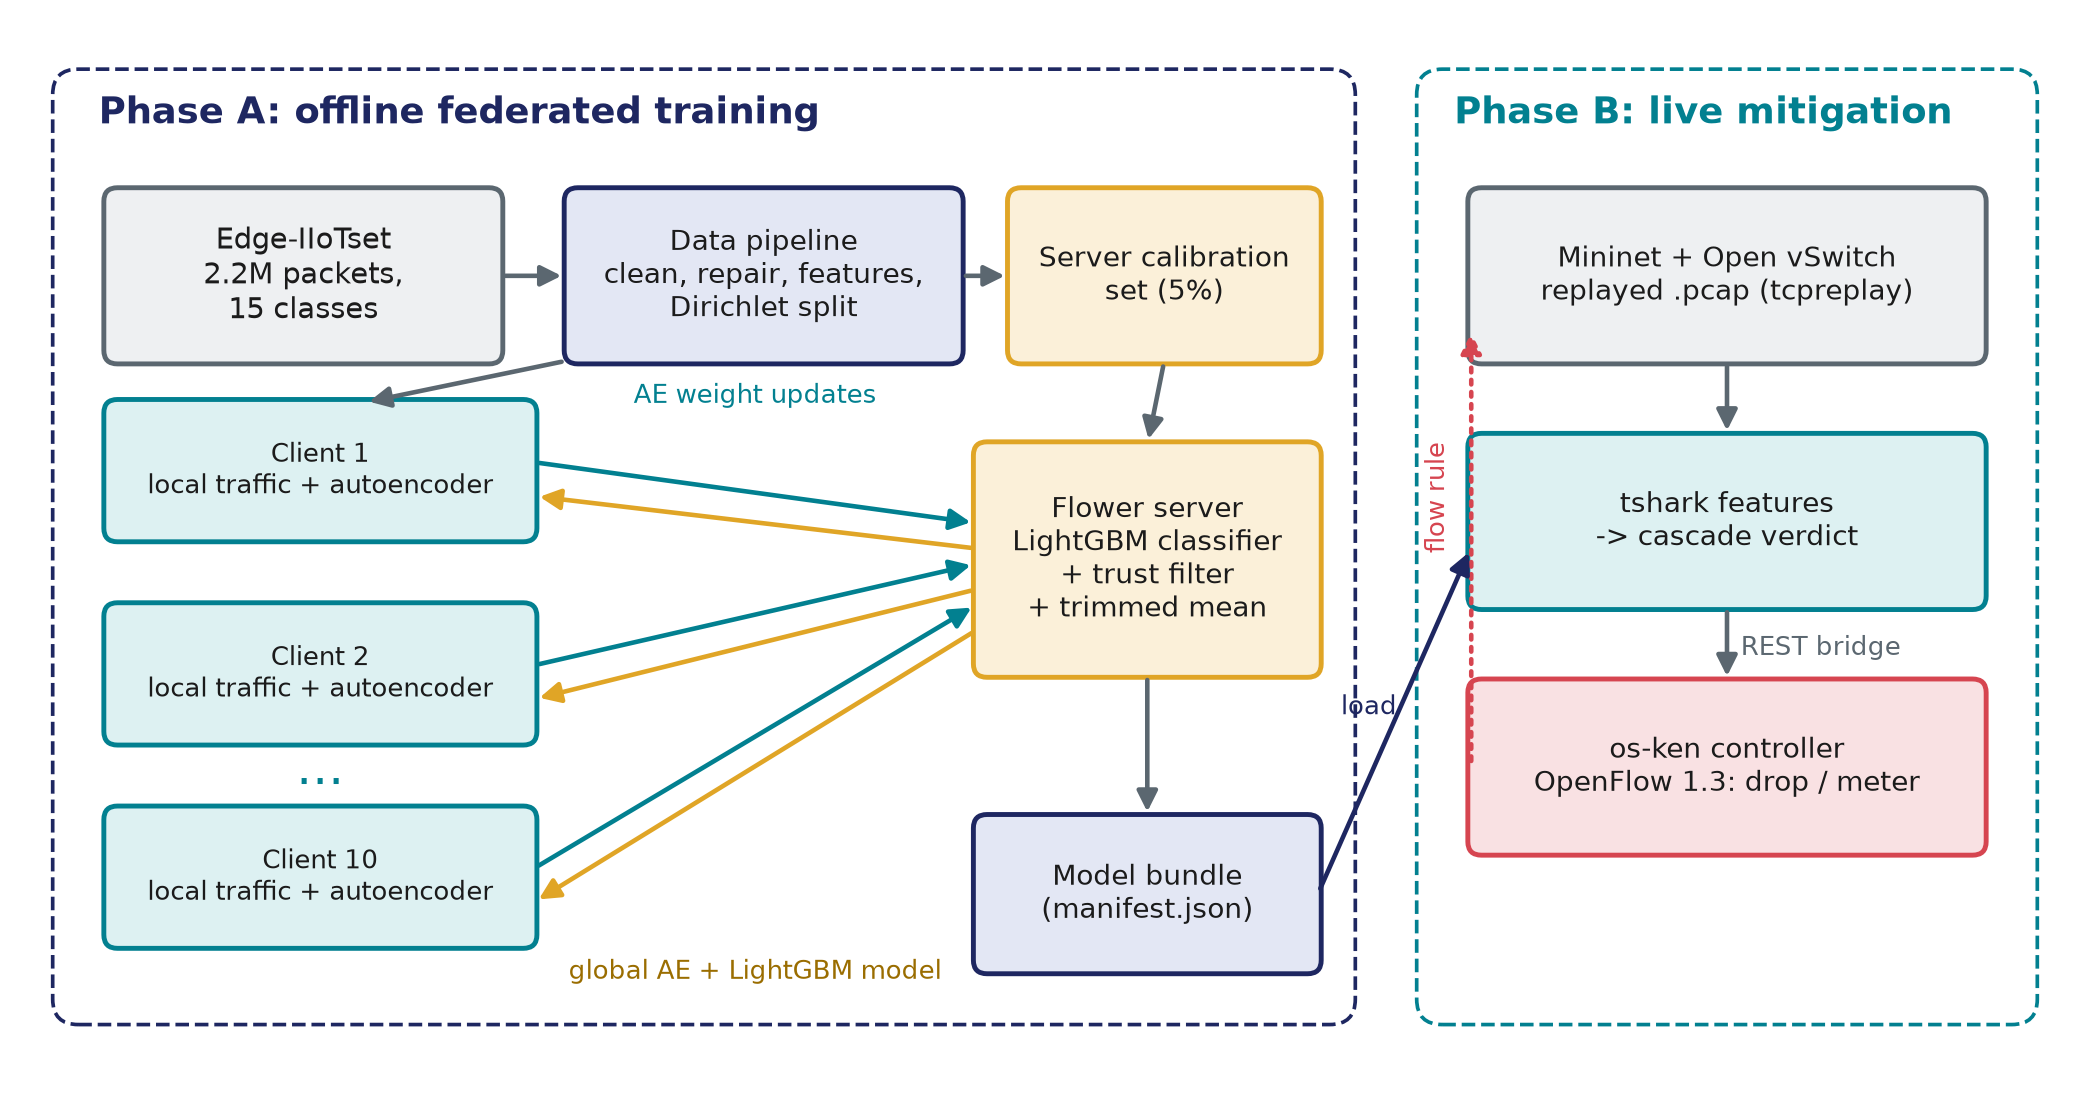
\includegraphics[width=\linewidth]{figures/high_level_design.png}
\caption{High-level design of FL-IDS}
\label{fig:hld}
\end{figure}

Four design decisions shape everything else.
\begin{enumerate}
  \item \textbf{Raw features for the classifier, normalised features for the autoencoder.} Trees split on raw values, so a client's own scaling cannot distort the shared classifier; the autoencoder needs scaled inputs and each client scales with its own statistics.
  \item \textbf{One decision rule.} The cascade rule exists in a single module and is used by the evaluation code, the dashboard and the SDN path, so the three cannot disagree.
  \item \textbf{Filtering on deltas.} The trust filter looks at each client's change to the weights, not at the weights, because honest weights differ a lot between non-IID clients but their updates point the same way.
  \item \textbf{A self-describing bundle.} Phase B rebuilds everything from the bundle's manifest, never from the current configuration, and refuses a bundle whose saved thresholds do not match the saved weights.
\end{enumerate}

\section{Module/Component Design}
The code is a Python package, \texttt{fl\_ids}, with one sub-package per component. Table~\ref{tab:modules} lists them.
\begin{table}[H]
\centering
\scriptsize
\renewcommand{\arraystretch}{1.2}
\begin{tabular}{|>{\raggedright\arraybackslash}p{2.6cm}|>{\raggedright\arraybackslash}p{3.9cm}|>{\raggedright\arraybackslash}p{6.4cm}|}
\hline
\textbf{Sub-package} & \textbf{Modules} & \textbf{Responsibility} \\ \hline
\texttt{data} & \texttt{pipeline}, \texttt{repair}, \texttt{features}, \texttt{sampling}, \texttt{synthetic} & Cleaning, MITM repair, one-hot encoding, service-port, content and flow features, connection-grouped splitting and the Dirichlet partition; a synthetic generator for tests \\ \hline
\texttt{models} & \texttt{boosting}, \texttt{boosting\_update}, \texttt{autoencoder}, \texttt{cascade}, \texttt{dl\_classifier} & First-stage classifier and its incremental update, the autoencoder, the shared cascade rule, and the deep-learning baseline \\ \hline
\texttt{fl} & \texttt{client}, \texttt{server}, \texttt{strategy}, \texttt{launch}, \texttt{data\_io} & Flower client and server, the custom strategy, starting the processes, loading each client's shard \\ \hline
\texttt{robustness} & \texttt{trust\_filter}, \texttt{aggregation}, \texttt{attackers} & Cosine/MAD/EMA filter, clipping and trimmed mean, and the sign-flip and stealth test attackers \\ \hline
\texttt{sdn} & \texttt{topology}, \texttt{controller}, \texttt{bridge}, \texttt{feature\_extraction}, \texttt{live\_inference}, \texttt{demo\_io} & Mininet topology, os-ken OpenFlow 1.3 controller, Flask bridge, TShark-based feature extraction and per-host scoring \\ \hline
\texttt{orchestration} & \texttt{phase\_a}, \texttt{phase\_b}, \texttt{artifacts} & Phase A and Phase B entry points; saving and loading the model bundle \\ \hline
\texttt{eval} & 18 modules, including \texttt{ablation}, \texttt{poisoning\_sweep}, \texttt{zero\_day}, \texttt{adaptive\_attack}, \texttt{pruning}, \texttt{metrics} & Every experiment in Chapter~\ref{chap:results} and the metrics they share \\ \hline
\texttt{dashboard} & \texttt{app}, \texttt{data} & Streamlit view of training and mitigation state \\ \hline
\texttt{utils} & \texttt{config}, \texttt{journey}, \texttt{logging\_setup} & Configuration loading, stage timing (the ``journey''), logging \\ \hline
\end{tabular}
\caption{Packages and modules of FL-IDS}
\label{tab:modules}
\end{table}
Outside the package, \texttt{configs/} holds one YAML file per experiment, \texttt{tools/} holds the latency benchmark and similar one-off tools, and \texttt{tests/} holds the automated tests.

\section{Detailed Design}
\subsection{One federated round}
Figure~\ref{fig:round} (Chapter~\ref{chap:method}) shows the arithmetic; Figure~\ref{fig:seq} shows the order of messages. The server never sees a packet: it receives weights, a 50-bin histogram of reconstruction errors, and every third round at most 50 confirmed alerts per surviving client.
\begin{figure}[H]
\centering
\begin{tikzpicture}[
  font=\scriptsize,
  life/.style={thick, dashed, gray},
  head/.style={draw, rounded corners=2pt, minimum width=2.4cm, minimum height=0.6cm, align=center, fill=gray!10},
  msg/.style={-{Stealth[length=5pt]}, thick},
  note/.style={font=\tiny, fill=white, inner sep=1pt}
]
\node[head] (S) at (0,0) {Server\\(strategy)};
\node[head] (C) at (5,0) {Client $i$};
\node[head] (B) at (9.8,0) {LightGBM\\(server-side)};
\draw[life] (S.south) -- ++(0,-7.4);
\draw[life] (C.south) -- ++(0,-7.4);
\draw[life] (B.south) -- ++(0,-7.4);
\draw[msg] (0,-1.1) -- node[note, above] {1. global autoencoder weights + classifier bytes} (5,-1.1);
\node[note, anchor=west] at (5.1,-1.9) {2. 5 local epochs on rows the classifier passes};
\draw[msg] (5,-2.7) -- node[note, above] {3. updated weights, error histogram} (0,-2.7);
\node[note, anchor=west] at (0.1,-3.3) {4. deltas, cosine to median, MAD, trust (EMA)};
\node[note, anchor=west] at (0.1,-3.8) {5. exclude outliers; clip; trimmed mean};
\node[note, anchor=west] at (0.1,-4.3) {6. new global weights};
\draw[msg] (5,-5.0) -- node[note, above] {7. every 3rd round: $\le$50 confirmed alerts} (0,-5.0);
\draw[msg] (0,-5.8) -- node[note, above] {8. continue or retrain on calibration set + alerts} (9.8,-5.8);
\draw[msg] (9.8,-6.6) -- node[note, above] {9. new classifier version} (0,-6.6);
\end{tikzpicture}
\caption{Order of messages in one federated round}
\label{fig:seq}
\end{figure}

\subsection{Cascade decision}
\begin{enumerate}
  \item The LightGBM classifier returns a class and its probability $p$.
  \item If the class is an attack and $p\ge0.7$ the label is final (the classifier's confidence is reported).
  \item Otherwise the autoencoder's reconstruction error $e$ is compared with the client's threshold $\tau_i$; $e>\tau_i$ gives \emph{anomalous}, with confidence $\mathrm{clip}(e/\tau_i-1,0,1)$.
  \item Anything else is benign.
\end{enumerate}
The module returns the label, the confidence and the stage that decided, which the bridge and the dashboard reuse. Figure~\ref{fig:cascade} (Chapter~\ref{chap:method}) is the flow chart of this rule.

\subsection{Trust filter and aggregation}
The filter is a pure function of the round's deltas and the previous trust scores: it returns which clients survive, why each excluded client was excluded (\texttt{mad\_outlier}, \texttt{opposes\_consensus} or \texttt{low\_trust}) and the new trust scores. Aggregation is a second pure function that takes the survivors' deltas, clips them and applies the trimmed mean. Keeping both free of Flower types made them testable on small arrays, and \texttt{TrustFilteredStrategy} only glues them to Flower's \texttt{aggregate\_fit}. If no client survives, the round is skipped.

\subsection{Phase B: from capture to rule}
\begin{enumerate}
  \item Mininet starts one host per federated client on one Open vSwitch switch; the os-ken controller connects over OpenFlow~1.3.
  \item \texttt{tcpreplay} sends a dataset capture from one host.
  \item TShark extracts the dataset's 61 fields; the same feature code as in training derives the 130 features.
  \item Each row is scored with that host's scaler and threshold; the most frequent non-benign label is the host's verdict, with its confidence and deciding stage.
  \item The Flask bridge receives \{device, classification, confidence, stage\}. Confidence $\ge0.85$ gives \emph{block}, $\ge0.5$ \emph{rate-limit}, otherwise \emph{allow}.
  \item The controller installs \texttt{priority=100,ip,nw\_src=}\emph{attacker}\texttt{ actions=drop} (or a meter), and the result is read back from the switch's flow table and saved with the verdict.
\end{enumerate}
Mininet needs root rights; it is started through a single permitted command whose parameters travel through a fixed file, so no other privileged command is exposed.

\subsection{Classes and interfaces that matter}
\begin{itemize}
  \item \textbf{Configuration}: a set of dataclasses (data, boosting, autoencoder, cascade and so on) loaded from YAML, so every value in a run is recorded with the run (\texttt{config.yaml} is copied into each run directory).
  \item \textbf{Bundle}: a loader that validates before use (Section~\ref{sec:datadesign}).
  \item \textbf{Cascade}: \texttt{flag\_attacks(mode, \ldots)} with the modes \texttt{boosting\_only}, \texttt{autoencoder\_only} and \texttt{cascade}, which is how the ablation and the latency benchmark call the same code path.
  \item \textbf{Journey}: a stage timer that records how long each step of a run took (loading and cleaning, bootstrap classifier and partition, federated training, threshold calibration, evaluation, saving the bundle).
\end{itemize}

\section{Data Design}\label{sec:datadesign}
\subsection{Dataset and splits}
Figure~\ref{fig:datasplit} shows how the dataset is divided. Rows are grouped into connections first; a connection is never divided.
\begin{figure}[H]
\centering
\begin{tikzpicture}[
  font=\scriptsize,
  box/.style={draw, rounded corners=2pt, align=center, minimum height=0.8cm, inner sep=3pt},
  arr/.style={-{Stealth[length=5pt]}, thick}
]
\node[box, text width=5.2cm] (raw) at (0,0) {Edge-IIoTset: 2{,}219{,}201 rows};
\node[box, text width=5.2cm, below=0.5cm of raw] (clean) {Cleaned, de-duplicated, 130 features:\\1{,}985{,}768 rows, 342{,}814 connections};
\node[box, text width=3.6cm, below left=0.7cm and -0.6cm of clean] (cal) {Server calibration set\\$\approx$5\% (71{,}853--79{,}866 rows)};
\node[box, text width=3.6cm, below right=0.7cm and -0.6cm of clean] (pool) {Federated pool\\$\approx$95\% (1{,}885{,}587--1{,}885{,}744 rows)};
\node[box, text width=3.2cm, below=0.7cm of pool, xshift=-2.2cm] (tr) {Client training\\(autoencoder)};
\node[box, text width=3.2cm, below=0.7cm of pool, xshift=1.2cm] (va) {Benign validation\\(threshold)};
\node[box, text width=3.2cm, below=0.7cm of pool, xshift=4.6cm] (te) {Client test slice\\(scoring)};
\draw[arr] (raw) -- (clean);
\draw[arr] (clean) -- (cal);
\draw[arr] (clean) -- (pool);
\draw[arr] (pool) -- (tr);
\draw[arr] (pool) -- (va);
\draw[arr] (pool) -- (te);
\end{tikzpicture}
\caption{How the dataset is divided; every connection goes to exactly one box}
\label{fig:datasplit}
\end{figure}
The pool is divided among $N$ clients with a Dirichlet($\alpha=0.3$) label skew, so some clients see almost no benign traffic (up to three of 20 clients had no benign validation rows in the main runs).

\subsection{Files written by a run}
\begin{table}[H]
\centering
\scriptsize
\renewcommand{\arraystretch}{1.2}
\begin{tabular}{|>{\raggedright\arraybackslash}p{4.6cm}|>{\raggedright\arraybackslash}p{8.4cm}|}
\hline
\textbf{File} & \textbf{Contents} \\ \hline
\texttt{boosting\_model.txt} & The LightGBM model in text form \\ \hline
\texttt{autoencoder\_weights.npz} & Final global autoencoder weights \\ \hline
\texttt{client\_normalization.npz} & Each client's mean, scale and threshold \\ \hline
\texttt{manifest.json} & Class names, the 130 feature names, input size, autoencoder shape, cascade settings, clip value, thresholds, held-out metrics, training summary (rounds, trust scores, survivors, classifier updates), seed, data set name, creation time and git commit \\ \hline
\texttt{journey.json} & Seconds spent in each stage of the run \\ \hline
\texttt{runs/.../phase\_a/} & Per-client logs and arrays, calibration arrays and the configuration used \\ \hline
\texttt{runs/.../phase\_b/} & Topology, bridge and controller logs, and \texttt{phase\_b\_result.json} with the verdict, the action and the flow table read back \\ \hline
\texttt{results/*.json} & One file per experiment (for example the latency benchmark) \\ \hline
\end{tabular}
\caption{Files that make up a model bundle and a run record}
\label{tab:files}
\end{table}

\subsection{Record layout}
A record is a vector of 130 numeric features. The first 91 are the dataset's own fields after dropping 16 columns and one-hot encoding seven nominal ones; one is the service port, 18 describe payload content and 20 describe the flow the packet belongs to (Section~\ref{sec:newfeat}). Class labels are stored as indices into the manifest's \texttt{class\_names} list, with Normal as the benign class. Identifiers (IP addresses, absolute time, ephemeral ports) are used only to group packets into flows and connections and are never stored as features.

\subsection{Bundle validation}
On load, Phase B recomputes every client's threshold from the saved weights and checks that it equals the saved threshold and rejects the bundle if they differ. This catches a bundle assembled from two different runs.
